%!TEX root = ../../../../memoria.tex
\subsection{\ordersEF}

	Por definición, una orden corresponde a una solicitud confirmada, en esta caso particular, desde un cliente para comprar un producto o servicio bajo unos términos y condiciones específicas. Es importante mencionar que el flujo de compra no ha terminado cuando el cliente a realizado el pago. Es en este escenario en donde surge el concepto de \orderFulfillmentCOM.
	Esta sección permite al encargado administrar las órdenes generadas por los clientes para posteriormente gestionarlas, conteniendo por lo tanto, toda la información necesaria para llevar a cabo dicho proceso.
	Dada la complejidad de operaciones que puede alcanzar \orderFulfillmentCOM, en la aplicación, está sección se ha simplificado a lo más fundamental.

	Al seleccionar las \ordersEF desde el panel de \dashboardEF, lo primero que se vera es la lista de todas las \ordersEF ingresadas por los clientes que se encuentran actualmente en el sistema. En la \refFigura{figure:dashboard:orders:grid} se ve la pantalla de \ordersEF.


	\begin{figure}[h!]
		\centering
		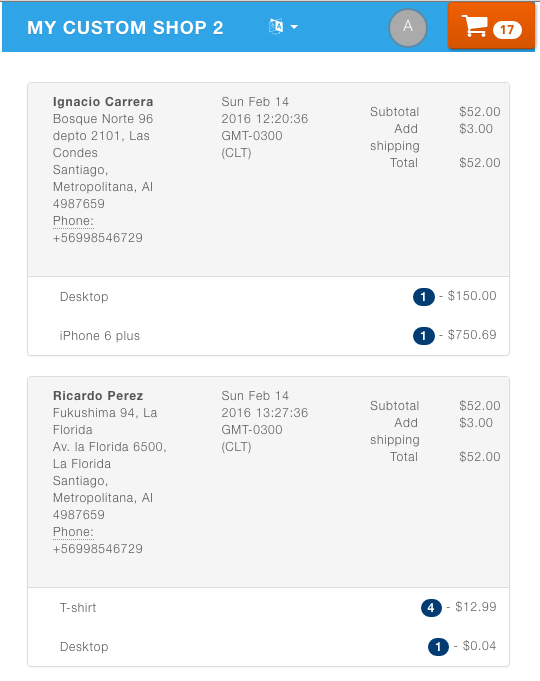
\includegraphics[width=0.6\textwidth]{figuras/orders/grid/main.png}
		\caption{Vista general de todas las \ordersEF ingresadas por clientes.}
		\label{figure:dashboard:orders:grid}
	\end{figure}

	La Componente visual de una \orderEF se encuentra áltamente influenciada por la interfaz de detalle de una \orderEF del sitio \dealextremeNAME. Con el fín de simplificar espació, se tomó el resumen de la compra y se movió desde el costado inferior derecho, al superior derecho. La \refFigura{figure:dashboard:orders:single_order} muestra la interfáz de una orden.

	\begin{figure}[h!]
		\centering
		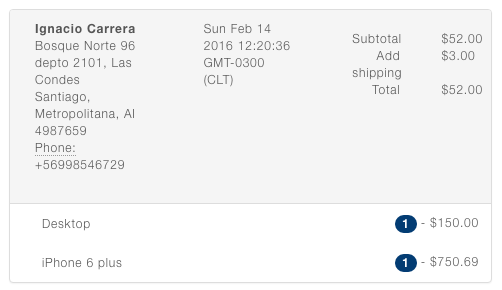
\includegraphics[width=0.7\textwidth]{figuras/orders/grid/order.png}
		\caption{Orden ingresada por un cliente.}
		\label{figure:dashboard:orders:single_order}
	\end{figure}

% 	Cada una de estas órdenes está disponible para realizar acciones sobre ellas. Estas acciones radican principalmete en cambiar el estado actual de la orden. El detalle de la orden se ve en la \refFigura{figure:dashboard:orders:orderInfo}.
% %TODO agregar mas información sobre la orden.
% 	\begin{figure}[h!]
% 		\centering
% 		\includegraphics[width=0.6\textwidth]{figuras/dashboard/orders/orderInfo.png}
% 		\caption{Detalle de orden ingresada por un cliente.}
% 		\label{figure:dashboard:orders:orderInfo}
% 	\end{figure}